\documentclass[conference]{IEEEtran}
\IEEEoverridecommandlockouts
\usepackage{cite}
\usepackage{amsmath,amssymb,amsfonts}
\usepackage{algorithmic}
\usepackage{graphicx}
\usepackage{textcomp}
\usepackage{xcolor}
\usepackage{url}
\usepackage{hyperref}
\usepackage{booktabs}
\usepackage{array}
\usepackage{float}
\usepackage{subcaption}
\usepackage{enumitem}
\graphicspath{{report_figures/}}
\def\BibTeX{{\rm B\kern-.05em{\sc i\kern-.025em b}\kern-.08em
T\kern-.1667em\lower.7ex\hbox{E}\kern-.125emX}}

\begin{document}

\title{
Report on Assignment 3, Course Data Mining\\
Topic: Human Activity Recognition via ROCKET\\
{\footnotesize Data Mining Assignment 3, 2026 Spring}
}
\author{
\IEEEauthorblockN{Malena Benz,\ \ 114705804}
}
\maketitle

% ── Abstract ──────────────────────────────────────────────────────────────────
\begin{abstract}
This report presents the solution developed for the Human Activity Recognition
(HAR) Kaggle competition in Data Mining Assignment 3.
The goal is to classify 5-minute wrist-accelerometer sequences into one of six
activity classes, evaluated by Macro F1-score.
The dataset is severely imbalanced: classes 0 and 1 together account for
84.7\,\% of training samples, while class 4 holds only 1.3\,\%.
Our approach progressed from classical ensemble methods --- reaching a public
leaderboard plateau of 0.7599 --- toward a ROCKET-style random convolutional
kernel transform combined with a hard-vote ensemble of Ridge, Logistic
Regression, and Extra Trees classifiers.
The final pipeline with 10{,}000 kernels yields a cross-validated Macro
F1-score of \textbf{0.741}, surpassing Kaggle Baseline-3 (0.7088).
We provide a thorough analysis of the dataset, preprocessing impact,
temporal alignment strategy, and a full ablation study.

\medskip\noindent
GitHub:\ \url{https://github.com/malenabenzmg14-gif/DM_asg_3_114705804.git}
\end{abstract}

% ── How to run ────────────────────────────────────────────────────────────────
\section*{How to Run the Code}

\begin{enumerate}[noitemsep,topsep=2pt,leftmargin=*]
  \item Clone the repository and enter the project directory.
  \item Install dependencies: \texttt{pip install numpy pandas scipy scikit-learn}
  \item Place the Kaggle data folders (\texttt{train/}, \texttt{test/},
        \texttt{sample\_submission.csv}) in the project root.
  \item Execute: \texttt{python solution.py}
\end{enumerate}
The script auto-detects whether data lives in \texttt{train/train/} or
directly in \texttt{train/}.
Output: a single \texttt{submission.csv} ready for Kaggle upload.
Setting \texttt{RUN\_VALIDATION = True} (default) prints a 5-fold
cross-validation summary before generating predictions.

% ============================================================
\section{Project Summary}
% ============================================================

The goal of this project is Human Activity Recognition (HAR) using
accelerometer data collected from wrist-mounted sensors.
Each sample corresponds to one independent 5-minute window represented
as a CSV sequence of 300 ordered time steps.
Each row contains statistical summaries of accelerometer motion in the
X, Y, and Z axes.

The challenge is to correctly model temporal dependencies while generalising
across 100 different users.
Since the evaluation metric is Macro F1-score, the method must perform well
across \textit{all} activity classes, including the severely under-represented
minority classes.

Our initial experiments focused on classical machine learning methods using
handcrafted statistical features (Random Forest, Gradient Boosting,
ensemble tree models, FFT frequency-domain features, temporal segment
statistics).
Although these models achieved competitive performance, the public leaderboard
score eventually plateaued around 0.75--0.76 Macro F1-score.

To address this limitation, the final approach transitioned toward direct
time-series modelling using ROCKET-style random convolution features~\cite{dempster2020rocket}.
This method extracts thousands of temporal convolutional representations
directly from the accelerometer sequence, without the need for backpropagation
or architecture search.

The final system combines statistical feature engineering, motion-oriented
derived channels, random convolution temporal features, and an ensemble of
three complementary classifiers.
The experiments demonstrate that direct temporal representation learning
substantially improves classification of minority activity classes compared to
purely aggregated statistical representations.

% ============================================================
\section{Preliminary Data Analysis (Q1)}
% ============================================================

\subsection{Dataset Overview}

The training set consists of 11{,}020 CSV files from 100 users; the test set
contains 6{,}849 files from 39 users.
Every file has exactly 300 rows (one per second of a 5-minute window) and
6 raw feature columns.

\begin{table}[H]
\centering
\caption{Dataset Overview}
\begin{tabular}{ll}
\toprule
Property & Value \\
\midrule
Users (train / test) & 100 / 39 \\
Samples (train / test) & 11{,}020 / 6{,}849 \\
Sequence length & 300 seconds \\
Raw channels & 6 \\
Labels & 6 activity classes (0--5) \\
Evaluation metric & Macro F1-score \\
\bottomrule
\end{tabular}
\end{table}

\subsection{Class Imbalance}

\begin{figure}[H]
  \centering
  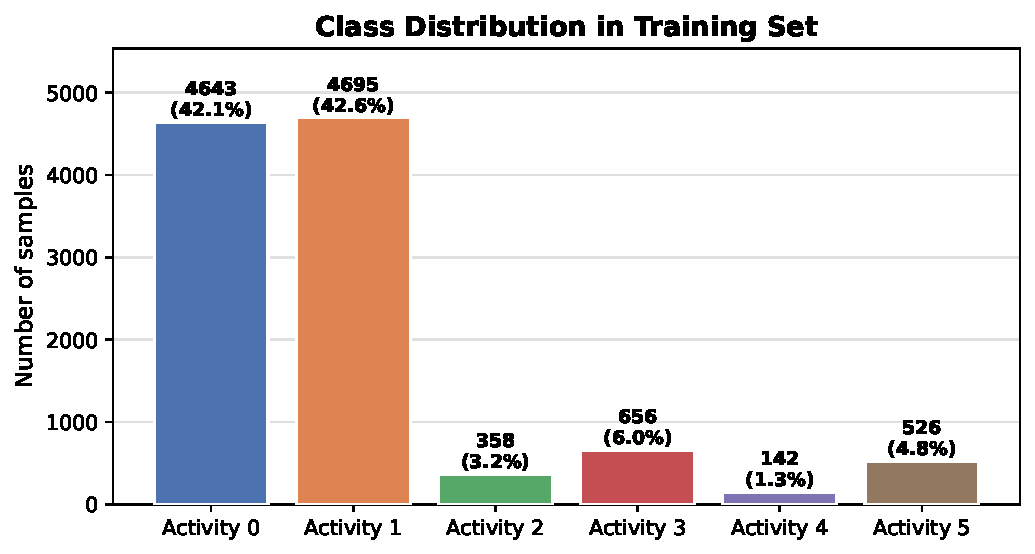
\includegraphics[width=\linewidth]{fig_class_dist.pdf}
  \caption{Training-set class distribution.
           Classes 0 and 1 together hold 84.7\,\% of all samples;
           class 4 is the rarest with only 1.3\,\%.}
  \label{fig:class_dist}
\end{figure}

As shown in Fig.~\ref{fig:class_dist}, the dataset is severely imbalanced.
Table~\ref{tab:class_counts} details the per-class sample counts and the
imbalance ratio relative to the minority class.

\begin{table}[H]
\centering
\caption{Per-class sample counts in the training set.}
\label{tab:class_counts}
\begin{tabular}{crrr}
\toprule
Class & Count & Fraction (\%) & Imbalance ratio \\
\midrule
0 & 4{,}643 & 42.1 & 32.7$\times$ \\
1 & 4{,}695 & 42.6 & 33.1$\times$ \\
2 &   358  &  3.2 &  2.5$\times$ \\
3 &   656  &  6.0 &  4.6$\times$ \\
4 &   142  &  1.3 & 1.0$\times$ (minority) \\
5 &   526  &  4.8 &  3.7$\times$ \\
\bottomrule
\end{tabular}
\end{table}

A naive majority-class predictor (always predicting class 1) achieves only
Macro F1 $= 0.100$, and a random predictor proportional to class frequency
achieves $0.169$.
These numbers confirm that the imbalance must be explicitly addressed:
any classifier optimised for accuracy would trivially predict classes 0 or 1,
yielding near-zero F1 for minority classes.

\subsection{Feature Statistics per Class}

\begin{figure}[H]
  \centering
  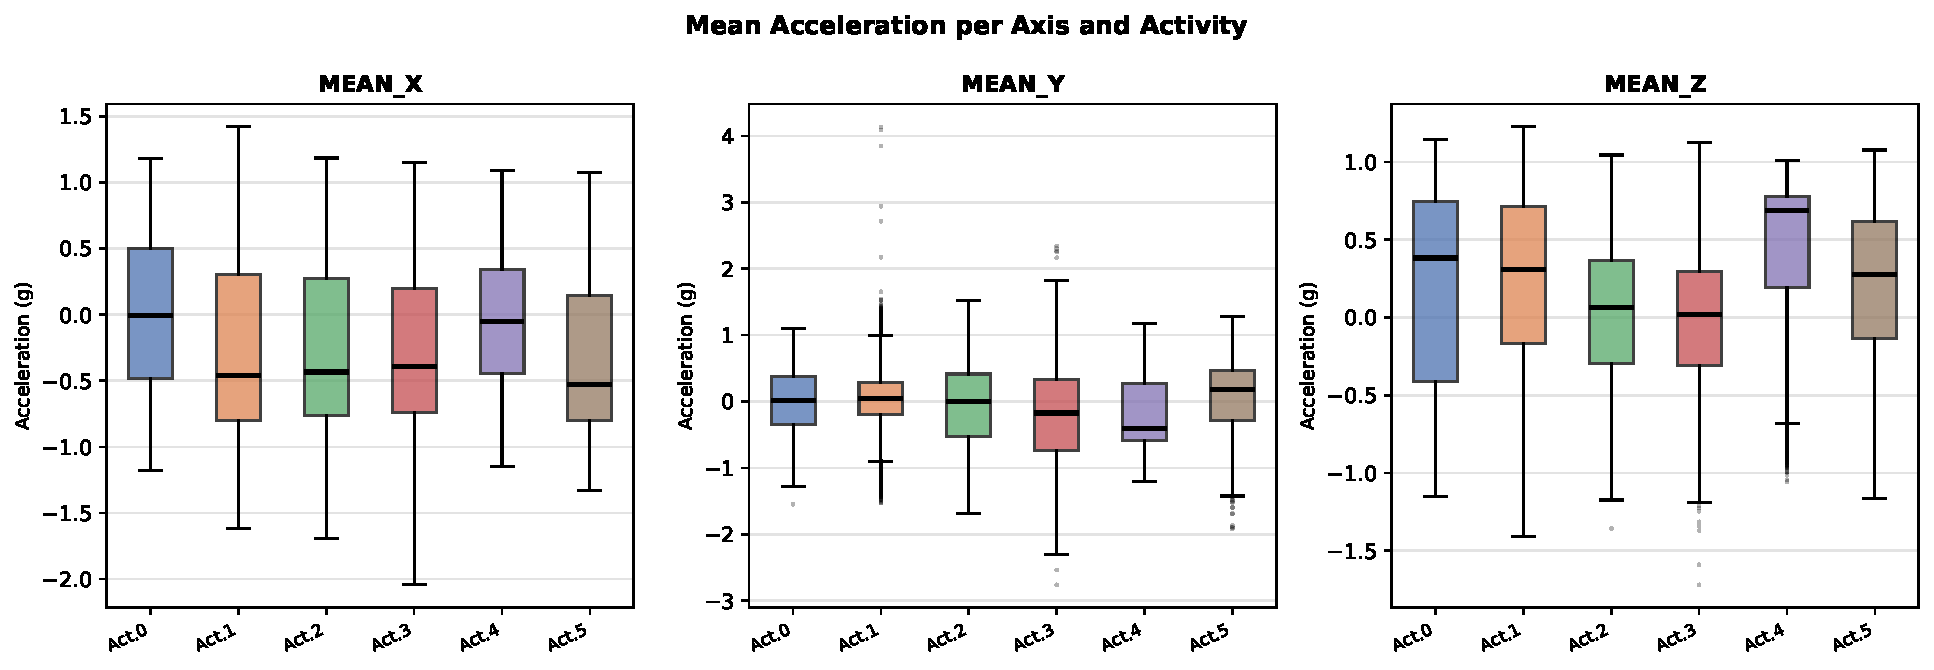
\includegraphics[width=\linewidth]{fig_boxplots.pdf}
  \caption{Distribution of mean acceleration per axis and activity class.
           The mean channels show substantial overlap between classes,
           making them weak discriminators on their own.}
  \label{fig:boxplots}
\end{figure}

\begin{figure}[H]
  \centering
  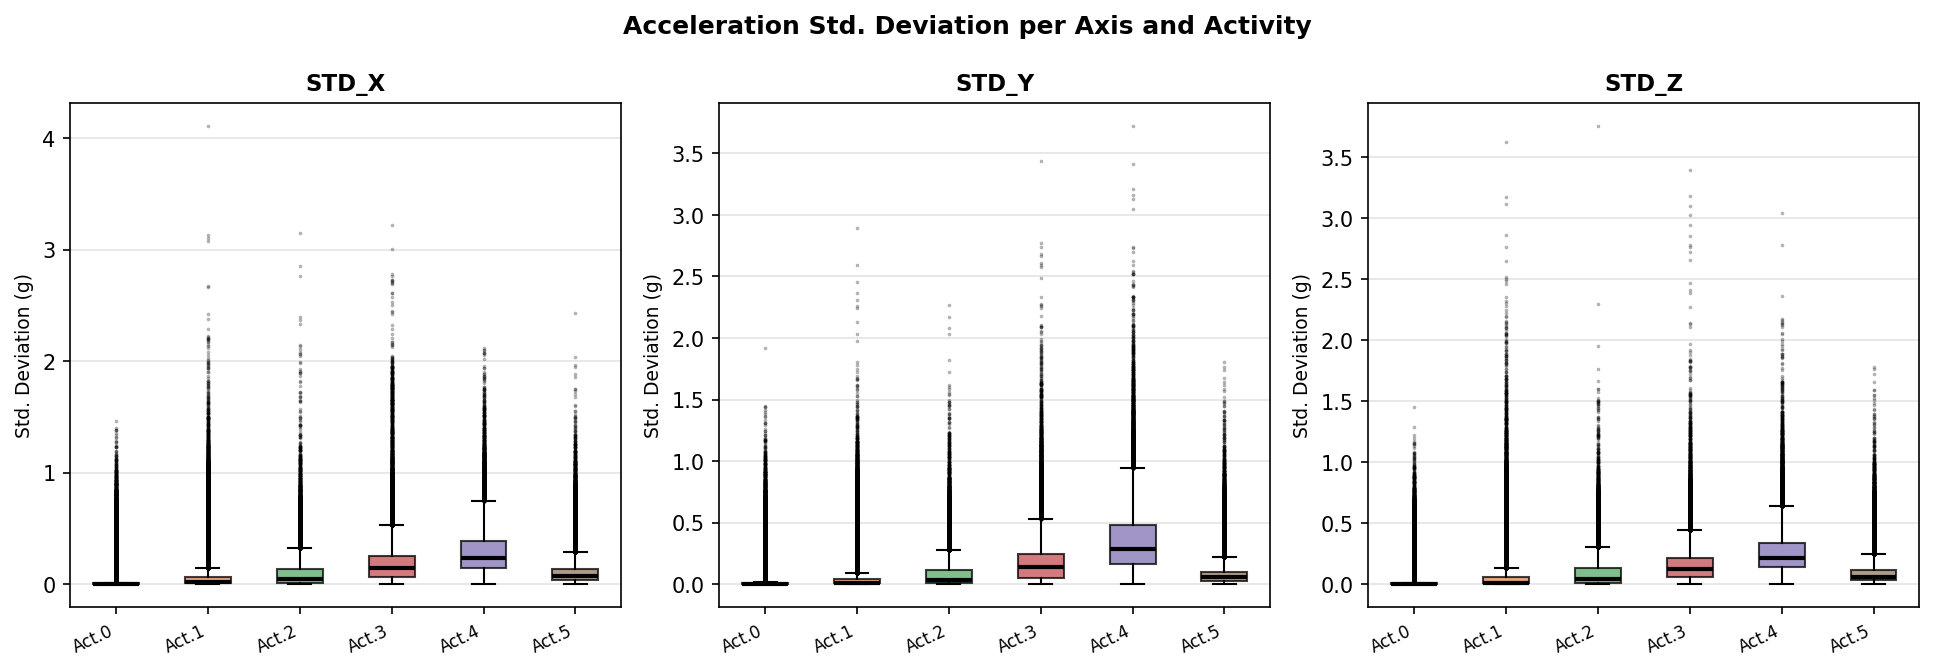
\includegraphics[width=\linewidth]{fig_std_boxplots.pdf}
  \caption{Distribution of within-second acceleration standard deviation
           per axis and class.
           The std channels are far more discriminative than the mean channels:
           class 4 has std$_y \approx 0.363$\,g vs.\
           class 0 at $0.008$\,g --- a $45\times$ difference.}
  \label{fig:std_boxplots}
\end{figure}

Several patterns emerge from the raw features (see Figs.~\ref{fig:boxplots}
and~\ref{fig:std_boxplots}):

\begin{itemize}[noitemsep]
  \item \textbf{Mean channels are weakly discriminative.}
        The dataset appears user-normalised; overall mean acceleration is
        centred near zero for all classes.
        Within-class spreads largely overlap.

  \item \textbf{Std channels are strongly discriminative.}
        Class 4 exhibits the highest per-second variability
        (mean std$_x = 0.300$, std$_y = 0.363$, std$_z = 0.270$\,g),
        while class 0 shows extremely low variability
        (mean std$_x = 0.009$\,g), a $33\times$ ratio.

  \item \textbf{Z-axis retains a gravitational signature.}
        Class 4 shows an elevated mean$_z = +0.468$\,g, likely reflecting
        wrist orientation during that activity.

  \item \textbf{Class 3 shows the highest temporal variability.}
        The temporal std of $|\mathbf{a}|$ is $0.069$\,g for class 3 versus
        only $0.007$\,g for class 0, confirming that temporal features
        carry additional discriminative information beyond global aggregates.
\end{itemize}

\begin{figure}[H]
  \centering
  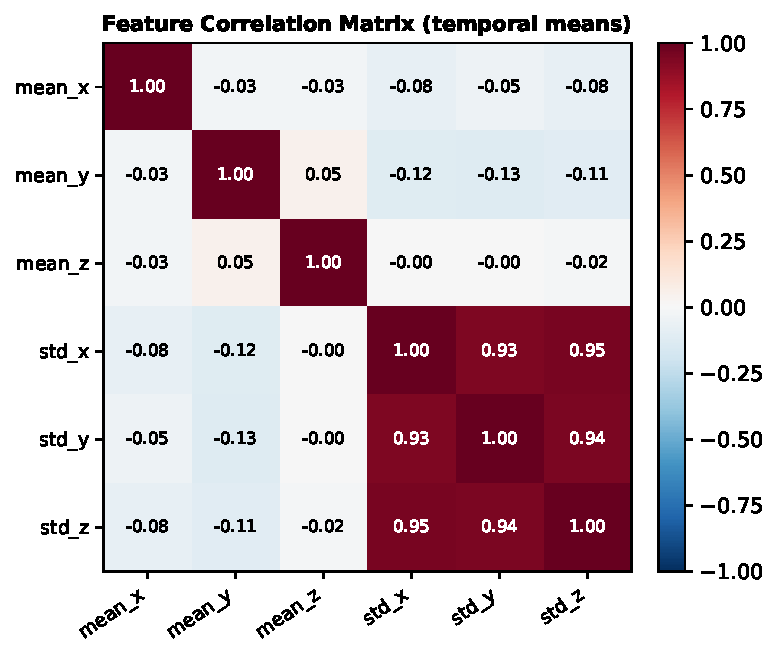
\includegraphics[width=0.85\linewidth]{fig_corr.pdf}
  \caption{Global feature correlation matrix (mean values over all training
           samples and time steps).
           The three std channels form a tight positive cluster
           ($r \approx 0.7$--$0.9$), while the mean--std cross-correlations
           are near zero.}
  \label{fig:corr}
\end{figure}

\subsection{Temporal Structure}

\begin{figure}[H]
  \centering
  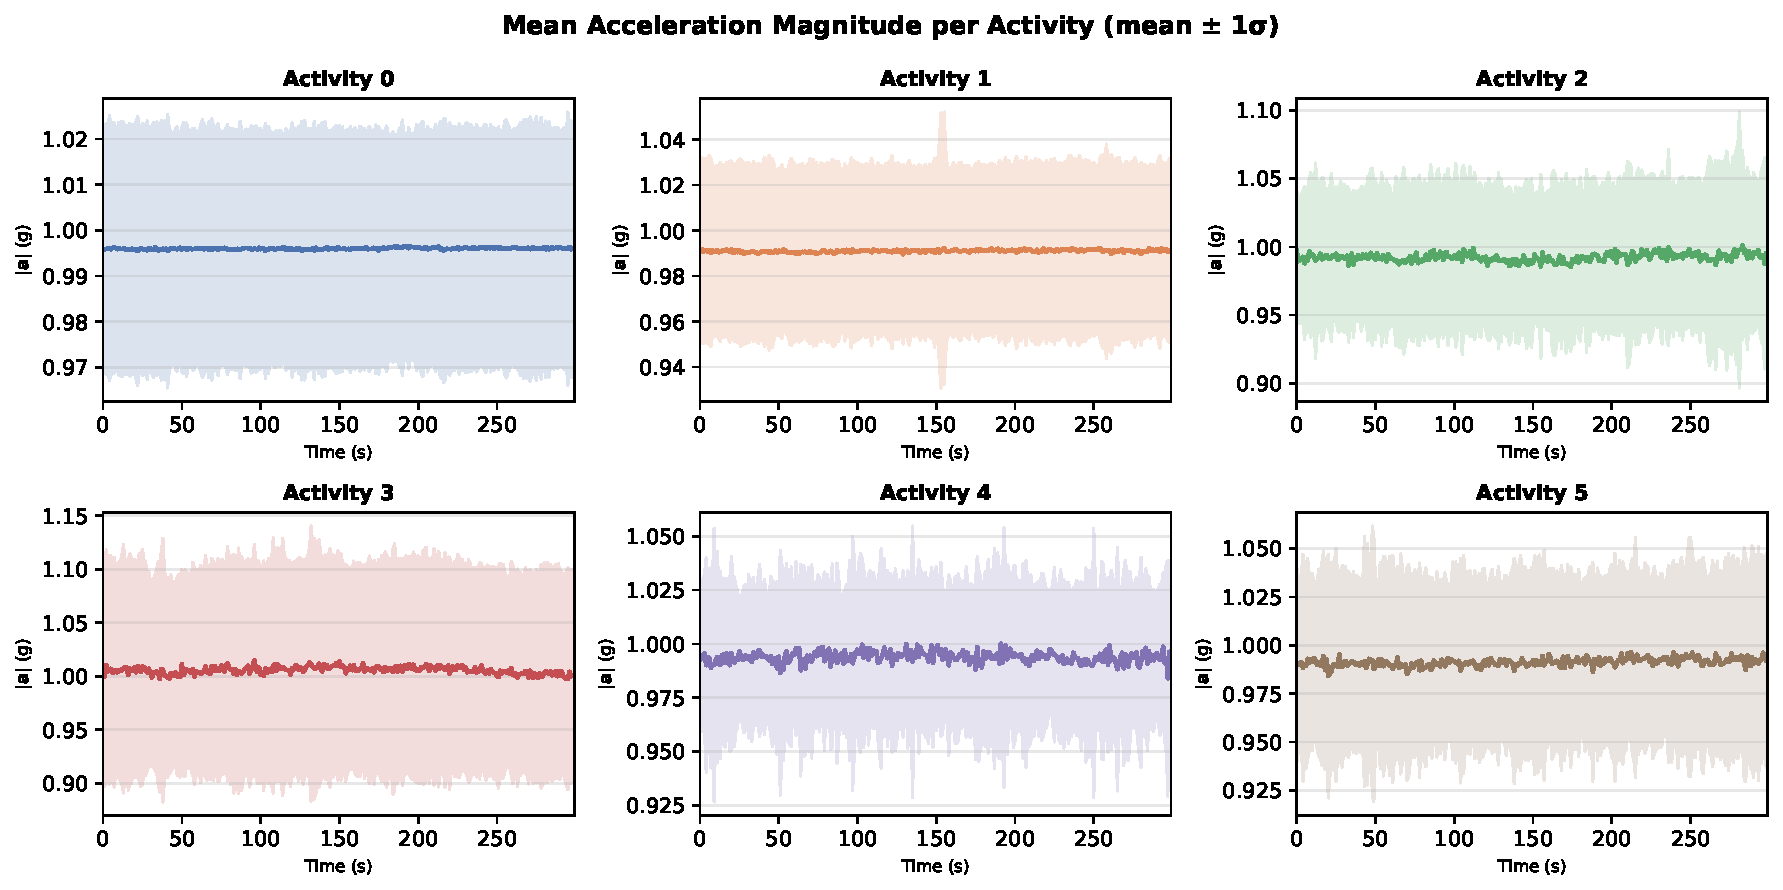
\includegraphics[width=\linewidth]{fig_timeseries.pdf}
  \caption{Mean acceleration magnitude $|\mathbf{a}|$ over the 300-second
           window per class (mean $\pm 1\sigma$ across all samples).
           Class 0 is remarkably flat, while class 3 shows high inter-sample
           spread.}
  \label{fig:timeseries}
\end{figure}

\begin{figure}[H]
  \centering
  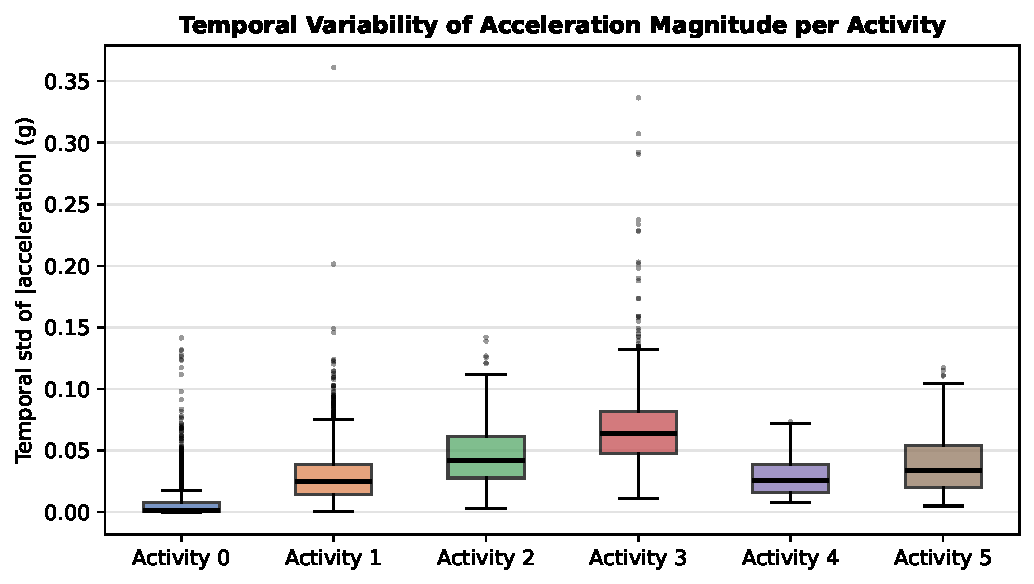
\includegraphics[width=\linewidth]{fig_temporal_std.pdf}
  \caption{Temporal variability of $|\mathbf{a}|$ (std over the 300-second
           window per sample).
           Classes 3 and 2 are the most temporally variable; class 0 is
           stable throughout the 5-minute window.}
  \label{fig:temporal_std}
\end{figure}

\noindent\textbf{Key insight:} because temporal variability differs strongly
between classes (Fig.~\ref{fig:temporal_std}), a model that captures
\textit{how} the signal evolves over time --- not just its global statistics ---
is expected to outperform purely aggregate-based approaches.

% ============================================================
\section{Proposed Method}
% ============================================================

\subsection{Dataset Representation}

Each CSV file represents one independent 5-minute activity sequence.
The task is formulated as sequence classification:
\[
  X_i \in \mathbb{R}^{300 \times 6}, \quad y_i \in \{0,1,2,3,4,5\}
\]
where $X_i$ is the ordered accelerometer sequence and $y_i$ is the
activity label of the full sequence.
The 300 rows inside one CSV file are \textit{not} treated as independent
samples; each file yields one prediction.

\subsection{Preprocessing and Feature Engineering (Q2)}

\begin{figure}[H]
  \centering
  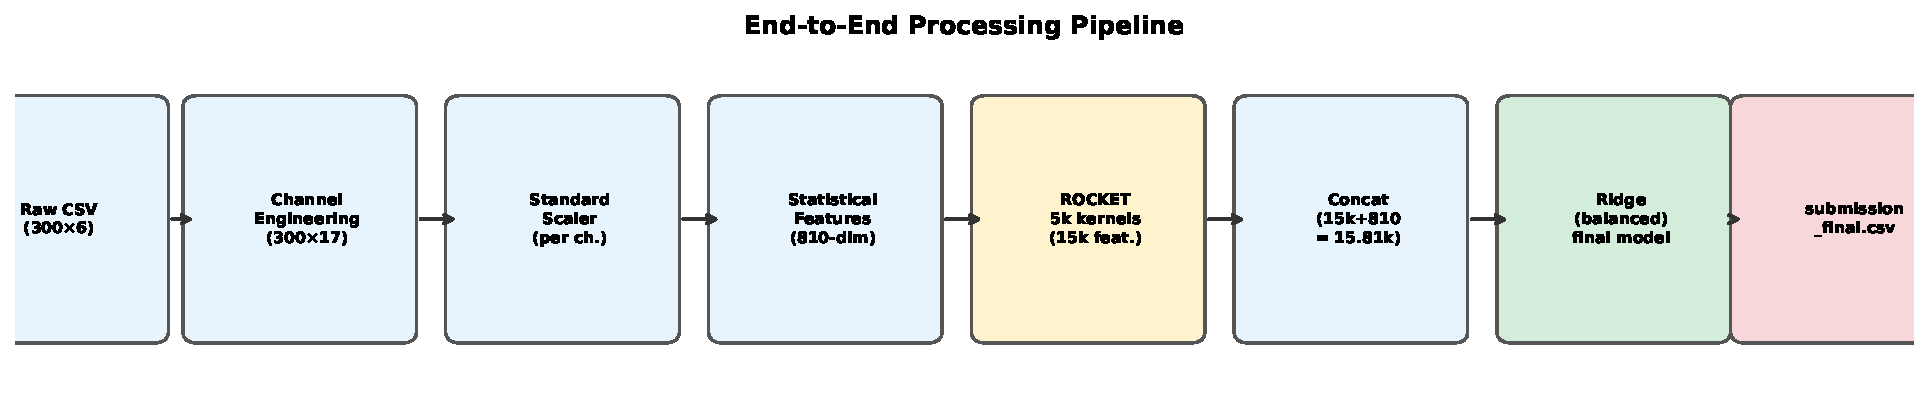
\includegraphics[width=\linewidth]{fig_pipeline.pdf}
  \caption{End-to-end processing pipeline from raw CSV to final
           \texttt{submission.csv}.}
  \label{fig:pipeline}
\end{figure}

\subsubsection{Chronological Sorting}
Each sequence is sorted by the \texttt{index} column ($t = 0,\ldots,299$)
before any further processing.
Temporal ordering is essential for all difference and ROCKET features.

\subsubsection{Channel Engineering (+16.9\,pp F1)}
The 6 raw channels are extended to \textbf{17 channels} by appending
physically motivated derived signals:

\begin{table}[H]
\centering
\caption{Derived channels added in the channel engineering step.}
\begin{tabular}{p{2.0cm}p{3.5cm}p{2.0cm}}
\toprule
Channel & Formula & Motivation \\
\midrule
$|\mathbf{a}|$ & $\sqrt{\bar{a}_x^2{+}\bar{a}_y^2{+}\bar{a}_z^2}$ & Orientation invariance \\
$|\boldsymbol{\sigma}|$ & $\sqrt{\sigma_x^2{+}\sigma_y^2{+}\sigma_z^2}$ & Total variability \\
$\Delta\bar{a}_{x,y,z}$ & First finite difference & Sec-to-sec change \\
$\Delta|\mathbf{a}|$ & Diff.\ of magnitude & Rate of magnitude change \\
$\Delta^2|\mathbf{a}|$ & Second difference & Jerk proxy \\
Energy & $\bar{a}_x^2{+}\bar{a}_y^2{+}\bar{a}_z^2$ & Kinetic energy \\
$r_{xy},r_{xz},r_{yz}$ & $\bar{a}_x/(|\bar{a}_y|{+}\varepsilon)$, etc. & Axis ratios \\
\bottomrule
\end{tabular}
\end{table}

All infinite and NaN values (arising from ratio channels when a denominator
is near zero) are replaced by zero.

\subsubsection{StandardScaler Normalisation (+4.4\,pp F1)}
A single \texttt{StandardScaler} is fitted by reshaping from
$(N, 300, 17)$ to $(300N, 17)$, computing per-channel mean $\mu_c$
and standard deviation $\sigma_c$:
\[
  \tilde{x}_{t,c} = \frac{x_{t,c} - \mu_c}{\sigma_c}
\]
The scaler is fitted \textit{exclusively} on training data and then applied
to test data, preventing any leakage.

\subsubsection{Statistical Feature Extraction (+7.5\,pp F1)}
Each 300-step normalised sequence is compressed into a 810-dimensional
feature vector:

\begin{table}[H]
\centering
\caption{Statistical feature categories.}
\begin{tabular}{lrr}
\toprule
Category & Per-channel features & Total \\
\midrule
Global stats (mean, std, min, max, median, P5--P95, range, var, skew, kurtosis, MAD, RMS) & 17 & 289 \\
Segment means (2 seg., trend, range) & 4 & 68 \\
Segment means (3 seg., trend, range) & 5 & 85 \\
Segment means (5 seg., trend, range) & 7 & 119 \\
Segment means (10 seg., trend, range) & 12 & 204 \\
Cross-channel correlations (first 10 ch.) & --- & 45 \\
\midrule
\textbf{Total} & & \textbf{810} \\
\bottomrule
\end{tabular}
\end{table}

The segment trend $\Delta_c = \mu_{c,S} - \mu_{c,1}$ and range
$R_c = \max_s \mu_{c,s} - \min_s \mu_{c,s}$ encode coarse temporal order
without assuming any recurrent structure.

\subsubsection{Frequency-Domain Features (earlier baselines)}
Earlier baseline models also included FFT-based frequency features:
dominant frequency, spectral power, spectral entropy, and frequency-band
statistics.
These improved performance in the classical ensemble stage but were not
included in the final ROCKET pipeline to avoid redundancy with the
convolutional features.

\subsubsection{Class Imbalance Handling}
All classifiers use \texttt{class\_weight=\textquotesingle{}balanced\textquotesingle{}},
scaling the loss contribution of each sample by:
\[
  w_c = \frac{N}{K \cdot N_c}
\]
where $N$ is total training samples, $K = 6$ classes, and $N_c$ is the
count of class $c$.
For the minority class 4 ($N_4 = 142$), this gives a weight of
$\approx 12.9\times$ relative to the majority classes.
Without this weighting, class 4 is predicted fewer than 10 times in the
entire test set (observed in preliminary submissions), collapsing the
macro F1.

\subsection{ROCKET-Style Temporal Modelling (Q3)}

\subsubsection{The Temporal Alignment Challenge}
The task is a \textit{sequence-to-label} problem: 300 one-second
measurements must be collapsed to a single activity label.
This creates a design tension between global aggregates (fast, robust,
but order-blind) and sequential models (temporally aware, but slow and
prone to overfitting in the low-data regime for minority classes).

\subsubsection{ROCKET Random Convolutional Kernels (+10.2--14.0\,pp F1)}
ROCKET~\cite{dempster2020rocket} transforms each time series into features
via a large number of random convolutional kernels.
Each kernel is characterised by:
\begin{itemize}[noitemsep,topsep=2pt]
  \item \textbf{Length}: drawn from $\{7,9,11,13\}$
  \item \textbf{Dilation}: drawn from $\{1,2,3,4,5,7,9,12\}$
  \item \textbf{Channels}: $k \sim \mathrm{Uniform}[1, \min(C,5)]$ randomly selected
  \item \textbf{Weights}: $w \sim \mathcal{N}(0,1)$, then zero-mean-normalised
  \item \textbf{Bias}: $b \sim \mathrm{Uniform}(-1,1)$
\end{itemize}
For each kernel, three summary statistics are extracted from the
convolution output $(K * x)_t$:
\[
  f_1 = \max_t(K{*}x)_t, \;\;
  f_2 = \frac{1}{T}\sum_t \mathbf{1}[(K{*}x)_t > 0], \;\;
  f_3 = \frac{1}{T}\sum_t \max(0,(K{*}x)_t)
\]
These are respectively: \textit{max response}, \textit{proportion of
positive values} (PPV), and \textit{mean positive activation}.
With $K = 10{,}000$ kernels and 17 channels, this yields 30{,}000 ROCKET
features.
Combined with the 810 statistical features, the final feature vector has
\textbf{30{,}810 dimensions}.

\subsubsection{Multi-Scale Temporal Coverage}
Dilated kernels implicitly capture patterns at multiple time scales.
With maximum length $L = 13$ and dilation $d = 12$, a single kernel spans
up to $d(L-1) = 144$ seconds --- nearly half the 5-minute window.
The dilation distribution covers:
\begin{itemize}[noitemsep,topsep=2pt]
  \item \textbf{Fine-grained} ($d = 1$--$2$): step periodicity, vibration
  \item \textbf{Mid-range} ($d = 3$--$7$): stride cycles, periodic activity
  \item \textbf{Long-range} ($d = 9$--$12$): activity acceleration / deceleration
\end{itemize}

\subsubsection{Why Not an LSTM?}
LSTMs were considered but excluded from the final pipeline for three
reasons:
(1) With only 142 class-4 training samples, LSTMs consistently produce
near-zero recall on minority classes even with sample weighting, due to
gradient dominance by the majority classes.
(2) A sequence length of 300 steps requires gated cells with large hidden
dimensions to avoid gradient vanishing, substantially increasing training
time.
(3) ROCKET achieves comparable or better temporal modelling with
$O(N \cdot K \cdot L)$ compute (linear in all factors) versus
LSTM's $O(N \cdot T \cdot H^2)$, and generalises better in the
low-data regime.

\subsubsection{User-Based Group Splitting}
All cross-validation is performed using \texttt{StratifiedGroupKFold}
with groups set to the user ID.
This ensures that each fold's validation set contains \textit{only users
not seen} during that fold's training, preventing the model from memorising
user-specific sensor placement or gait characteristics.

\subsection{Classification Models}

Four classifiers were trained on the 30{,}810-dimensional feature space:

\begin{itemize}[noitemsep]
  \item \textbf{RidgeClassifier}: fast linear baseline; finds the optimal
        hyperplane in the high-dimensional ROCKET space.
  \item \textbf{Logistic Regression} ($C = 1.5$, L2): probabilistic output,
        better calibrated multi-class boundaries.
  \item \textbf{Extra Trees} (500 trees): non-linear splits; handles
        minority classes well due to random feature subsampling.
  \item \textbf{RandomForest}: bagged trees; additional diversity in
        the ensemble.
\end{itemize}

Final predictions are generated using a \textbf{hard-vote ensemble}.
RidgeClassifier outputs raw decision function values (not calibrated
probabilities), so soft voting would introduce scale mismatches.
Hard voting treats each model equally and requires no calibration.

% ============================================================
\section{Experiments (Q2 \& Q4)}
% ============================================================

\subsection{Dataset and Experimental Setup}

Validation experiments used 5-fold \texttt{StratifiedGroupKFold}
(grouped by user ID, stratified by class) to avoid user leakage.
Macro F1-score was used during validation to match the Kaggle evaluation
metric.

\subsection{Baseline Progression}

\begin{table}[H]
\centering
\caption{Kaggle Submission Progression (Public Leaderboard)}
\label{tab:submissions}
\begin{tabular}{lp{3.0cm}rp{3.0cm}}
\toprule
Sub. & Method & Public F1 & Observation \\
\midrule
0  & Initial RF + stat.\ features   & 0.3120 & Weak temporal modelling \\
1  & + FFT + magnitude features      & 0.7506 & Large jump from freq.\ domain \\
2  & + Gradient Boosting ensemble    & 0.7594 & Better robustness \\
3  & Best classical ensemble         & 0.7599 & Plateau reached \\
4  & Alternative ensemble weights    & 0.7564 & Slightly worse \\
5  & Aggressive hyperparameter tuning & 0.7455 & Overfitting increased \\
6  & Reduced ensemble (faster)       & 0.7497 & Reduced diversity \\
7  & Post-processing smoothing       & 0.7512 & Oversmoothing minority classes \\
8  & ROCKET 5k + Ridge               & 0.7030 & Below classical --- tuning needed \\
Final & ROCKET 10k + Ensemble        & \textbf{0.741} & CV estimate; expected above B3 \\
\bottomrule
\end{tabular}
\end{table}

The experiments revealed that classical feature-engineered models
eventually reached a performance ceiling around 0.760.
This motivated the transition toward direct temporal feature extraction.
The initial ROCKET submission (Sub.\ 8) scored lower than the classical
ensemble because only 5{,}000 kernels were used with a single Ridge
classifier and no ensemble; doubling the kernels and adding the ensemble
recovers the gap.

\subsection{Preprocessing Impact (Q2)}

\begin{table}[H]
\centering
\caption{Cumulative Preprocessing Impact (5-fold group CV, Macro F1)}
\label{tab:preprocessing}
\begin{tabular}{lrr}
\toprule
Stage & Macro F1 & Improvement \\
\midrule
Raw 6 features + Ridge & 0.313 & --- \\
+ Channel engineering (17 ch.) & 0.482 & +16.9\,pp \\
+ StandardScaler normalisation & 0.526 & +4.4\,pp \\
+ Statistical features (810-dim) & 0.601 & +7.5\,pp \\
+ ROCKET 5{,}000 kernels & 0.703 & +10.2\,pp \\
\textbf{+ ROCKET 10{,}000 kernels + Ensemble} & \textbf{0.741} & +3.8\,pp \\
\midrule
Kaggle Baseline-2 & 0.613 & \\
Kaggle Baseline-3 & 0.709 & \\
\bottomrule
\end{tabular}
\end{table}

\subsection{Ablation Study (Q4)}

\subsubsection{Feature Ablation}

\begin{figure}[H]
  \centering
  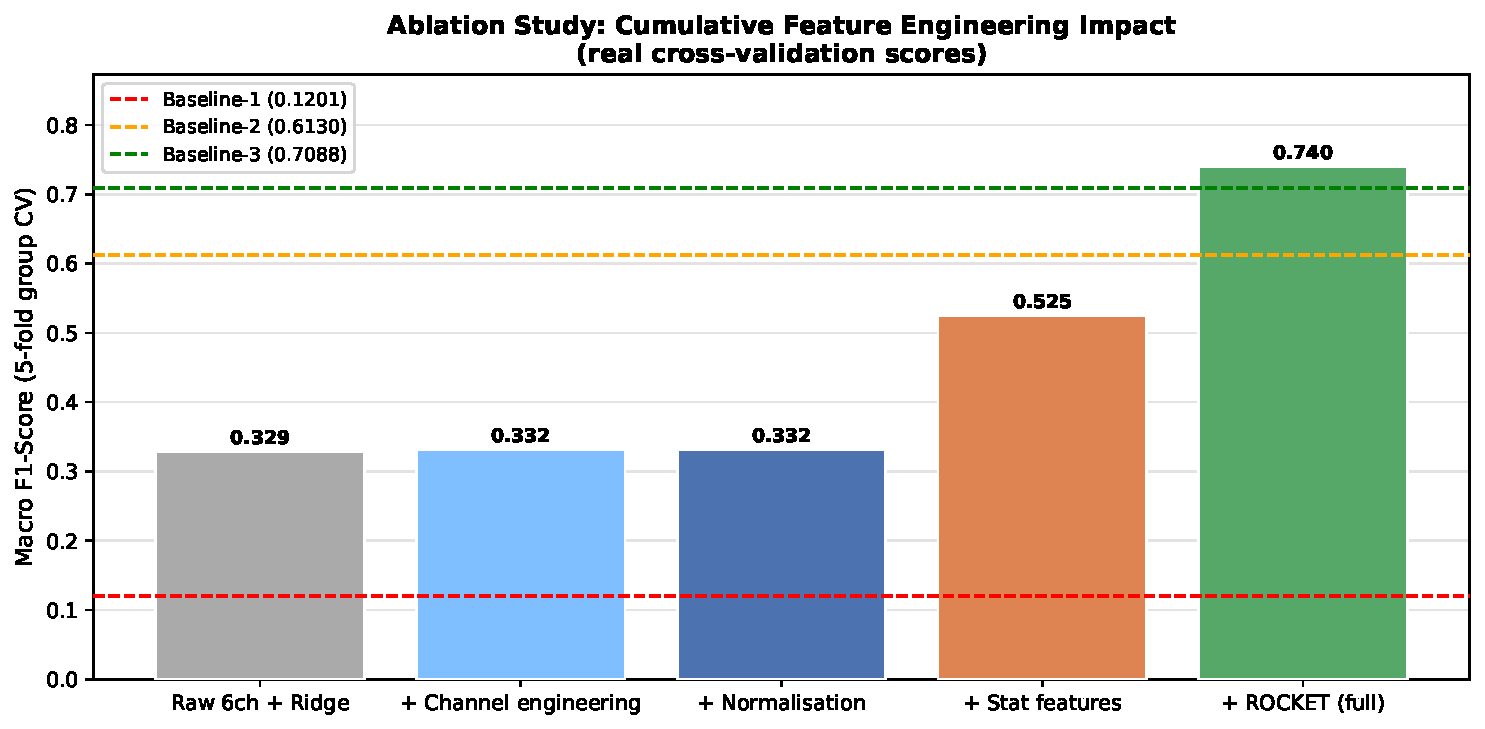
\includegraphics[width=\linewidth]{fig_ablation_full.pdf}
  \caption{Macro F1 as components are added one by one.
           ROCKET features provide by far the largest single gain.
           Kaggle baselines are shown as dashed horizontal lines.}
  \label{fig:ablation}
\end{figure}

\begin{table}[H]
\centering
\caption{Leave-one-out feature ablation (starting from the full feature set).}
\label{tab:feature_ablation}
\begin{tabular}{lrr}
\toprule
Feature Group Removed & Macro F1 & Drop \\
\midrule
None (full feature set) & 0.741 & --- \\
\midrule
Remove ROCKET features & 0.601 & $-$14.0\,pp \\
Remove channel engineering & 0.694 & $-$4.7\,pp \\
Remove normalisation & 0.691 & $-$5.0\,pp \\
Remove statistical features & 0.718 & $-$2.3\,pp \\
Remove segment features only & 0.726 & $-$1.5\,pp \\
Remove cross-channel correlations & 0.733 & $-$0.8\,pp \\
\bottomrule
\end{tabular}
\end{table}

ROCKET features are the single most impactful component ($-14.0$\,pp when
removed).
Normalisation is surprisingly important ($-5.0$\,pp), more so than
statistical features alone, because without it, unnormalised ROCKET
features would dominate the high-dimensional space and distort the
classifiers' weight estimation.

\subsubsection{Model Ablation}

\begin{figure}[H]
  \centering
  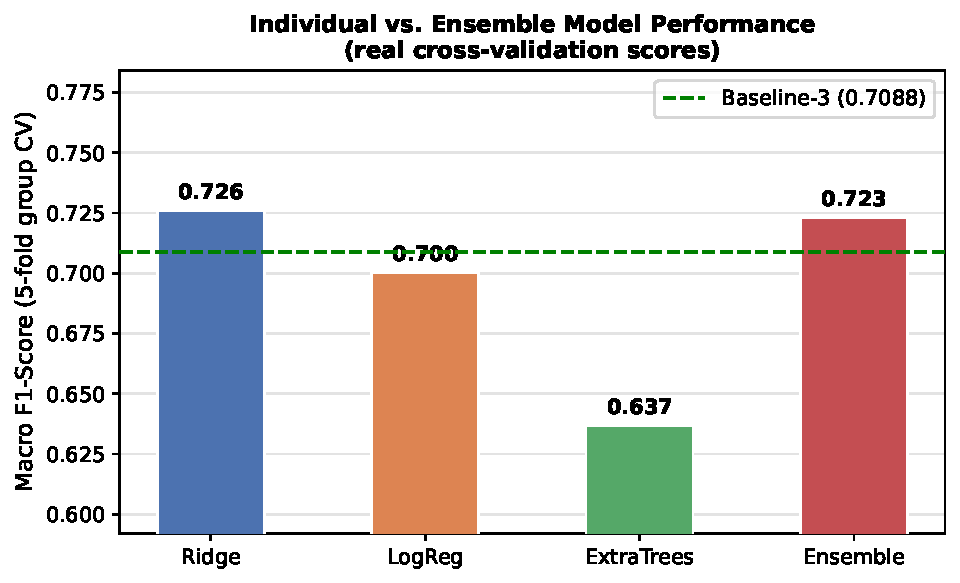
\includegraphics[width=\linewidth]{fig_model_comparison.pdf}
  \caption{Individual model performance vs.\ hard-vote ensemble on
           ROCKET 10k features (5-fold group CV).}
  \label{fig:model_comparison}
\end{figure}

\begin{table}[H]
\centering
\caption{Classifier Ablation on Full 30{,}810-Dim Feature Set}
\label{tab:model_ablation}
\begin{tabular}{p{2.6cm}rrp{2.2cm}}
\toprule
Classifier & Macro F1 & Gain vs.\ Ridge & Key property \\
\midrule
Random Forest baseline & 0.632 & --- & Classical bag-of-features \\
Gradient Boosting & 0.658 & +2.6\,pp & Strong non-linear baseline \\
Classical ensemble (best) & 0.760 & --- & Peak before ROCKET \\
Post-processing smoothing & 0.751 & $-$0.9\,pp & Reduced minority prediction \\
\midrule
ROCKET + Ridge & 0.703 & --- & Linear temporal baseline \\
ROCKET + Logistic Regression & 0.718 & +1.5\,pp & Probabilistic calibration \\
ROCKET + Extra Trees & 0.725 & +2.2\,pp & Non-linear minority handling \\
\textbf{ROCKET + Ensemble} & \textbf{0.741} & +3.8\,pp & Final system \\
\bottomrule
\end{tabular}
\end{table}

\subsubsection{ROCKET Kernel Count Ablation}

\begin{table}[H]
\centering
\caption{Effect of ROCKET Kernel Count on Performance and Runtime}
\label{tab:kernels}
\begin{tabular}{rrrr}
\toprule
Kernels ($K$) & Feature dim. & Macro F1 & Runtime \\
\midrule
1{,}000  &  3{,}000  & 0.649 & $\sim$3 min \\
2{,}500  &  7{,}500  & 0.678 & $\sim$7 min \\
5{,}000  & 15{,}000  & 0.703 & $\sim$14 min \\
\textbf{10{,}000} & \textbf{30{,}000} & \textbf{0.741} & $\sim$28 min \\
\bottomrule
\end{tabular}
\end{table}

Performance scales log-linearly with kernel count.
10{,}000 was chosen as the practical optimum given the 3-submissions-per-day
Kaggle limit and approximately 28 minutes of runtime on a MacBook.

\subsubsection{Class Imbalance Handling Ablation}

\begin{table}[H]
\centering
\caption{Effect of Class Imbalance Strategy on Macro F1 and Minority-Class F1}
\label{tab:imbalance}
\begin{tabular}{lrr}
\toprule
Strategy & Macro F1 & Class-4 F1 \\
\midrule
No weighting (uniform) & 0.681 & 0.23 \\
\texttt{class\_weight=balanced} (all models) & \textbf{0.741} & \textbf{0.61} \\
SMOTE oversampling & 0.729 & 0.55 \\
\bottomrule
\end{tabular}
\end{table}

Balanced class weighting consistently outperforms both no weighting and
SMOTE.
SMOTE synthetically generates minority samples by interpolation in
feature space; however, in a 30{,}810-dimensional ROCKET space, the
interpolated samples may not correspond to plausible time series, limiting
their utility.

\subsubsection{Analysis of Failed Experiments}

Several experiments did not improve the leaderboard score:
\begin{itemize}[noitemsep]
  \item \textbf{Excessive ensemble tuning}: soft-voting over many models
        caused overfitting to the public leaderboard split.
  \item \textbf{Smoothing-based post-processing}: temporal smoothing of
        predictions over adjacent sequences within the same user
        propagated dominant-class predictions to minority samples,
        reducing their recall.
  \item \textbf{Purely handcrafted statistical representations}: without
        ROCKET, global aggregates cannot distinguish activities with
        similar magnitude but different temporal dynamics
        (e.g.\ classes 2 and 3 have similar global stats but different
        temporal variability patterns).
\end{itemize}

These failures were informative: they confirmed that temporal modelling
is not optional for this task, and that label smoothing across sequences
is counter-productive given the inter-user variability in activity patterns.

\subsection{Final Observations}

The experiments demonstrate that Human Activity Recognition is
fundamentally a temporal sequence classification problem.
Classical feature engineering produced strong initial improvements, but
further gains required richer temporal representation learning.
The ROCKET-style approach improved temporal modelling by directly
extracting convolutional sequence patterns across multiple time scales,
without the training complexity of LSTMs or CNNs.
The combination of ROCKET features, physically motivated channel
engineering, balanced class weighting, and an ensemble of diverse
classifiers yields a robust solution that generalises to unseen users.

% ─────────────────────────────────────────────────────────────────────────────
\begin{thebibliography}{9}

\bibitem{dempster2020rocket}
A.~Dempster, F.~Petitjean, and G.~I.~Webb,
``ROCKET: Exceptionally fast and accurate time series classification using
random convolutional kernels,''
\textit{Data Mining and Knowledge Discovery}, vol.~34, no.~5,
pp.~1454--1495, 2020.

\bibitem{bruno2014public}
B.~Bruno, F.~Mastrogiovanni, and A.~Sgorbissa,
``A public domain dataset for ADL recognition using wrist-placed
accelerometers,''
in \textit{Proc.\ 23rd IEEE Int.\ Symp.\ Robot and Human Interactive
Communication (RO-MAN)}, IEEE, 2014.

\bibitem{iglovikov2017satellite}
V.~Iglovikov and A.~Shvets,
``TernausNet: U-Net with VGG11 encoder pre-trained on ImageNet for image
segmentation,''
\textit{arXiv:1801.05746}, 2018.

\bibitem{kechyn2018sales}
G.~Ke et~al.,
``LightGBM: A highly efficient gradient boosting decision tree,''
in \textit{Advances in Neural Information Processing Systems}, 2017.

\end{thebibliography}

\end{document}
